\newpage
\slidetitle{1. Einleitung}
\section{Einleitung \\}
\paragraph{Prozedurale Generierung\\}
\begin{itemize}
	\item Konstruktion von 3D-Modellen durch computergenerierte Daten
	\item Benötigt eingeschränkten Eingriff durch Benutzer
	\item Generierung von Pflanzenmodellen ist ein wichtiger Bestandteil
	\item In dieser Arbeit: Konzentration auf die Generierung von Baumstrukturen
\end{itemize}

\newpage
\slidetitle{1. Einleitung - Prozedurale Generierung}
\begin{center}
	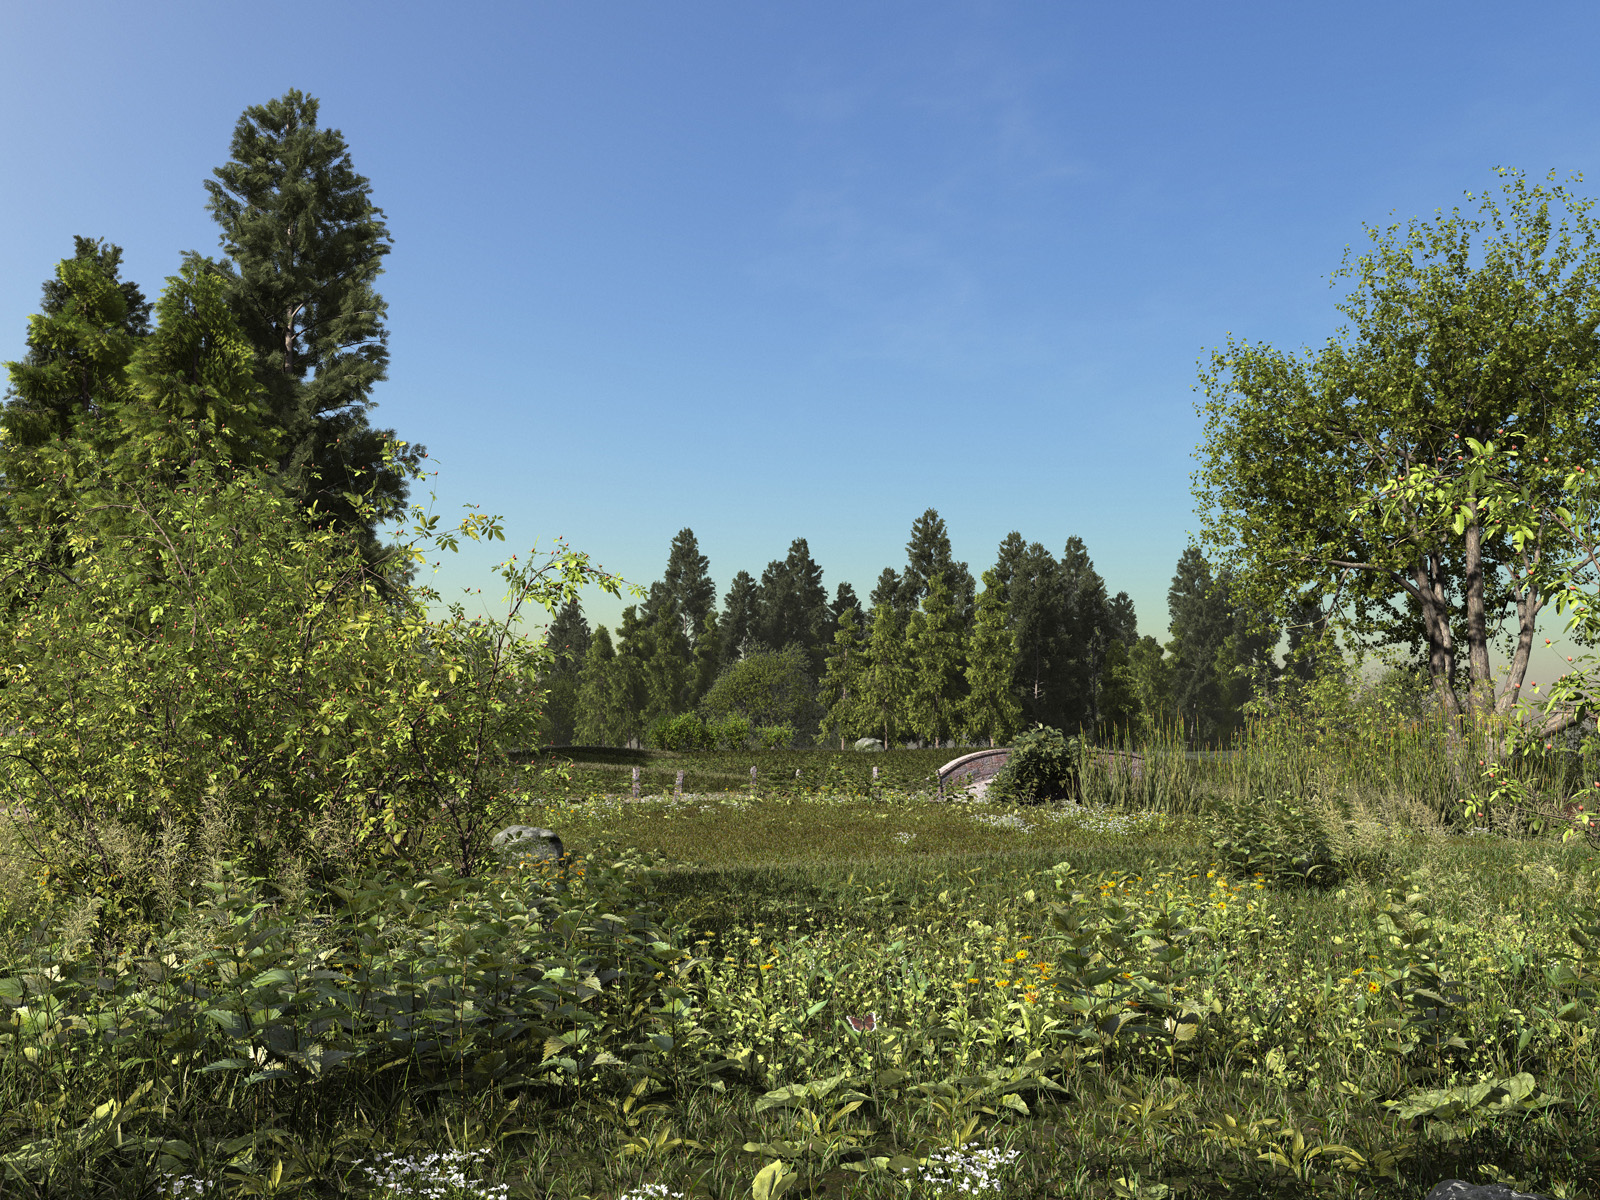
\includegraphics[height=.9\textheight]{images/greenXfrog_JanWalterSchliep.jpg}	
	
	Prozedural generierte Landschaftsszene. \cite{GreenOne:16}
\end{center}

\newpage
\slidetitle{1. Einleitung - Ansatz}
\paragraph{Ansatz\\}

\begin{itemize}
	\item Implementierung von zwei Verfahren zur prozeduralen Generierung von Baumstrukturen:
	\begin{itemize}
		\item Lindenmayer-Systeme
		\item Space Colonization Algorithmus
	\end{itemize}
	\item Verwendung des Frameworks der Unreal Engine 4
	\item Vereinfachte Darstellung von Ästen in Form von Zylindern
\end{itemize}

\newpage
\slidetitle{1. Einleitung - Unreal Engine 4}
\paragraph{Unreal Engine 4\\}

\begin{itemize}
	\item Sammlung von Softwarewerkzeugen
	\item In C++ programmiert mit frei einsehbarem Quellcode
	\item Inhalte werden in C++ oder Blueprint erstellt und leiten von Framework-Basisklassen ab
	\item Verfügbarkeit eines visuellen Editor:
	\begin{itemize}
		\item Ermöglicht die 
	\end{itemize}
\end{itemize}


\iffalse
\newpage
\slidetitle{1. Einleitung - Bisherige Arbeiten}
\paragraph{Bisherige Arbeiten}
\begin{center}
	\begin{minipage}[c]{0.45\textwidth}
		\centering
		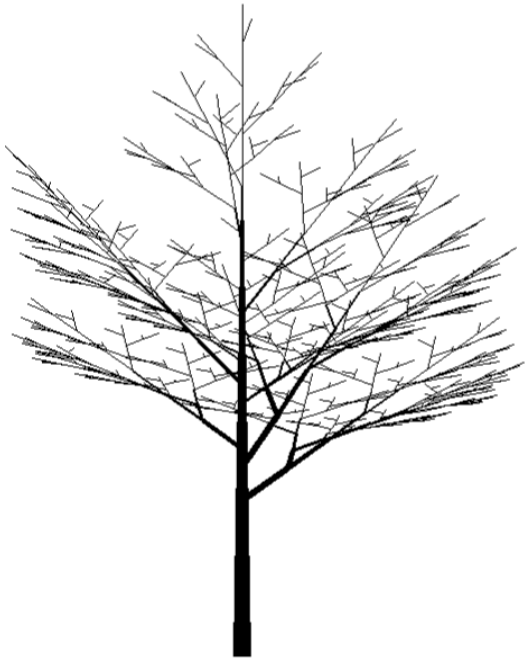
\includegraphics[height=0.6\textheight]{images/CH1_Honda1.png}
		
		Honda und Fisher \cite{ABOP:04}
	\end{minipage}
	\hspace{.05\textwidth}	
	\begin{minipage}[c]{0.45\textwidth}
		\centering
		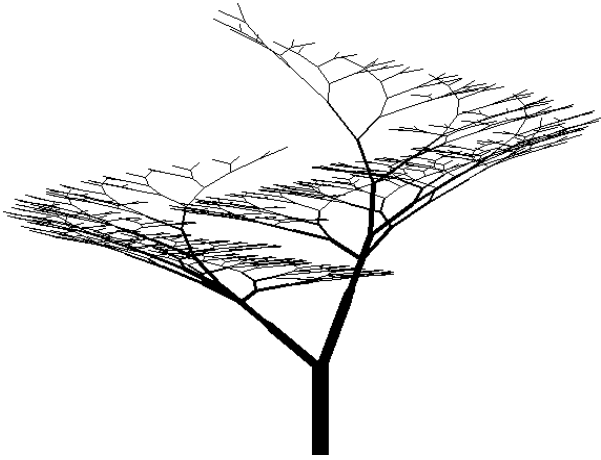
\includegraphics[height=0.6\textheight]{images/CH1_AonoKunii1.png}
		
		Aono und Kunii \cite{ABOP:04}
	\end{minipage}
\end{center}


\begin{center}
	\vfill
	\begin{minipage}[c]{0.45\textwidth}
		\centering
		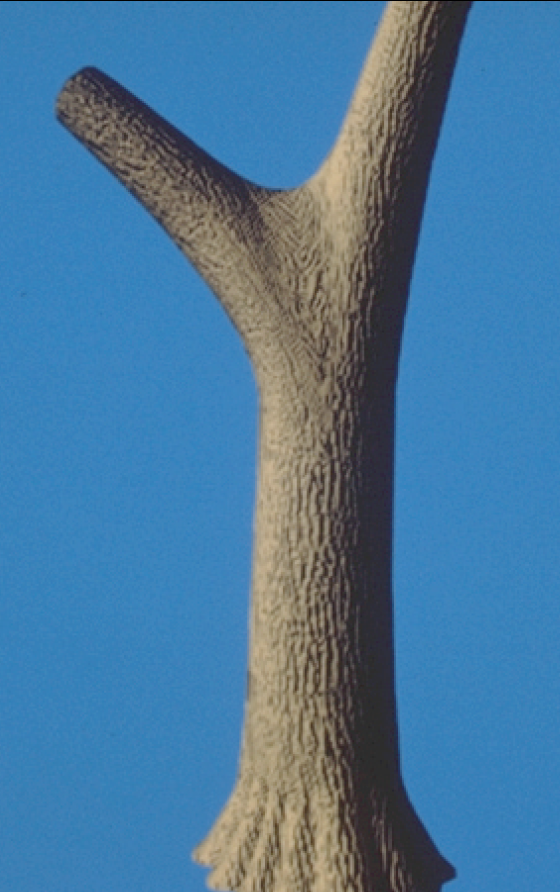
\includegraphics[height=0.6\textheight]{images/CH1_Bloomenthal1.png}
		
		Bloomenthal \cite{ABOP:04}
	\end{minipage}
	\hspace{.05\textwidth}	
	\begin{minipage}[c]{0.45\textwidth}
		\centering
		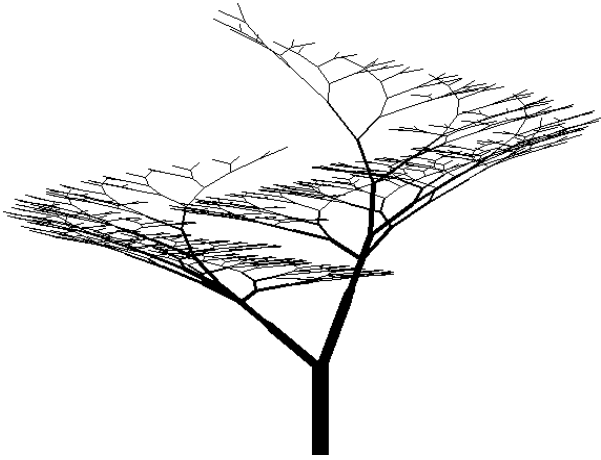
\includegraphics[height=0.6\textheight]{images/CH1_AonoKunii1.png}
		
		Aono und Kunii \cite{ABOP:04}
	\end{minipage}
\end{center}
\fi


	